\documentclass{amsart}

\usepackage{enumerate, amsmath, amsfonts, amssymb, amsthm, thmtools, wasysym, graphics, graphicx, xcolor, url, hyperref, hypcap, a4wide, pdflscape, multido, xargs, colortbl, multicol, multirow, calc, shuffle, hvfloat}
\hypersetup{colorlinks=true, citecolor=darkblue, linkcolor=darkblue}
%\usepackage[all]{xy}
\usepackage{tikz}
\usetikzlibrary{trees, decorations, decorations.markings, shapes, arrows, matrix, calc, fit, intersections, patterns, angles, cd}
\usepackage{tikz-qtree}
\usepackage{comment}
\usepackage{etex}
\usepackage{ulem}\normalem % to strike through a word
\usepackage[noabbrev,capitalise]{cleveref}
\setlength{\abovecaptionskip}{10pt}
\setlength{\belowcaptionskip}{5pt}
\usepackage[export]{adjustbox}

%\reserveinserts{50}
\graphicspath{{figures/}}
\makeatletter
\def\input@path{{figures/}}
\makeatother

%%%%%%%%%%%%%%%%%%%%%%%%%%%%%%%%%%%%%%

\title[Ornamentation lattices and intreeval hypergraphic lattices]{Ornamentation lattices and \\ intreeval hypergraphic lattices}

\author{Antoine Abram}
\address[A.~Abram]{}
\email{}
\urladdr{}

\author{Jose Bastidas}
\address[J.~Bastidas]{}
\email{}
\urladdr{}

\author{Félix Gélinas}
\address[F.~Gélinas]{}
\email{}
\urladdr{}

\author{Vincent Pilaud}
\address[V.~Pilaud]{Universitat de Barcelona \& Centre de Recerca Matemàtica, Barcelona}
\email{vincent.pilaud@ub.edu}
\urladdr{https://www.ub.edu/comb/vincentpilaud/}

\author{Andrew Sack}
\address[A.~Sack]{}
\email{}
\urladdr{}

\thanks{
VP was partially supported by the Spanish project PID2022-137283NB-C21 of MCIN/AEI/10.13039/501100011033 / FEDER, UE, by the Spanish--German project COMPOTE (AEI PCI2024-155081-2 \& DFG 541393733), by the Severo Ochoa and María de Maeztu Program for Centers and Units of Excellence in R\&D (CEX2020-001084-M), by the Departament de Recerca i Universitats de la Generalitat de Catalunya (2021 SGR 00697), and by the French--Austrian project PAGCAP (ANR-21-CE48-0020 \& FWF I 5788).
}


%%%%%%%%%%%%%%%%%%%%%%%%%%%%%%%%%%%%%%

% theorems
\newtheorem{theorem}{Theorem}[section]
\newtheorem{theoremA}{Theorem}
\renewcommand{\thetheoremA}{\Alph{theoremA}}
\crefname{theoremA}{Theorem}{Theorems}
\newtheorem{corollary}[theorem]{Corollary}
\newtheorem{proposition}[theorem]{Proposition}
\newtheorem{lemma}[theorem]{Lemma}
\newtheorem{conjecture}[theorem]{Conjecture}
\crefname{conjecture}{Conjecture}{Conjectures}
\newtheorem{conjectureA}{Conjecture}
\renewcommand{\theconjectureA}{\Alph{conjectureA}}
\crefname{conjectureA}{Conjecture}{Conjectures}
\crefname{conjectureA}{Conjecture}{Conjectures}

\theoremstyle{definition}
\newtheorem{definition}[theorem]{Definition}
\newtheorem{example}[theorem]{Example}
\newtheorem{remark}[theorem]{Remark}
\newtheorem{question}[theorem]{Question}
\newtheorem{notation}[theorem]{Notation}
\newtheorem{openproblem}[theorem]{Open problem}
\crefname{notation}{Notation}{Notations}


% newcommands
% math special letters
\newcommand{\R}{\mathbb{R}} % reals
\newcommand{\N}{\mathbb{N}} % naturals
\newcommand{\Z}{\mathbb{Z}} % integers
\newcommand{\I}{\mathbb{I}} % set of integers
\newcommand{\C}{\mathbb{C}} % set of summands
\renewcommand{\b}[1]{\boldsymbol{#1}} % bold
\renewcommand{\c}[1]{\mathcal{#1}} % bold
\newcommand{\cal}[1]{\mathcal{#1}} % cal

% math commands
\newcommand{\set}[2]{\left\{ #1 \;\middle|\; #2 \right\}} % set notation
\newcommand{\bigset}[2]{\big\{ #1 \;|\; #2 \big\}} % big set notation
\newcommand{\biggset}[2]{\bigg\{ #1 \;\bigg|\; #2 \bigg\}} % big set notation
\newcommand{\multiset}[2]{\left\{\!\!\left\{ #1 \;\middle|\; #2 \right\}\!\!\right\}} % multiset notation
\newcommand{\bigmultiset}[2]{\big\{\!\!\big\{ #1 \;|\; #2 \big\}\!\!\big\}} % big multiset notation
\newcommand{\ssm}{\smallsetminus} % small set minus
\newcommand{\dotprod}[2]{\langle #1 | #2 \rangle} % dot product
\newcommand{\symdif}{\triangle} % symmetric difference
\newcommand{\one}{{1\!\!1}} % the all one vector
\newcommand{\eqdef}{\mbox{\,\raisebox{0.2ex}{\scriptsize\ensuremath{\mathrm:}}\ensuremath{=}\,}} % :=
\newcommand{\defeq}{\mbox{~\ensuremath{=}\raisebox{0.2ex}{\scriptsize\ensuremath{\mathrm:}} }} % =:
\newcommand{\polar}{^\diamond} % polar
\newcommand{\simplex}{\triangle} % simplex
%\renewcommand{\implies}{\;\Rightarrow\;} % implies
\newcommand{\surjection}{\longrightarrow\mathrel{\mkern-22mu}\rightarrow\,}     
\newcommand{\bijection}{\longleftrightarrow}     

% operators
\DeclareMathOperator{\conv}{conv} % convex hull
\DeclareMathOperator{\cone}{cone} % cone hull
\DeclareMathOperator{\inv}{inv} % inversion set
\DeclareMathOperator{\tc}{tc} % transitive closure

% others
\newcommand{\fix}[1]{{\bf FIXME: }#1} % emphasis of a problem to FIX
\newcommand{\ie}{\textit{i.e.}~} % id est
\newcommand{\eg}{\textit{e.g.}~} % exempli gratia
\newcommand{\Eg}{\textit{E.g.}~} % exempli gratia
\newcommand{\aka}{\textit{aka.}~} % also known as
\newcommand{\viceversa}{\textit{vice versa}} % vice versa
\newcommand{\ordinal}{\textsuperscript{th}} % th for ordinals
\newcommand{\ex}[1]{^{\textrm{ex#1}}} % example
\newcommand{\para}[1]{\medskip\noindent\textbf{#1}} % paragraph
\newcommand{\subpara}[1]{\smallskip\noindent\textit{#1.}} % paragraph
\definecolor{darkblue}{rgb}{0,0,0.7} % darkblue color
\newcommand{\blue}[1]{{\color{blue} #1}} % blue
\newcommand{\red}[1]{{\color{red} #1}} % red
\newcommand{\darkblue}{\color{darkblue}} % darkblue command
\newcommand{\defn}[1]{\textsl{\darkblue #1}} % emphasis of a definition
\usepackage{todonotes}
\newcommand{\nantel}[1]{\todo[size=\tiny,color=red!30]{ #1 \\ \hfill --- N.}\,}
\newcommand{\Nantel}[1]{\todo[inline,color=red!30]{#1 \\ \hfill --- N.}}
\newcommand{\vincent}[1]{\todo[size=\tiny,color=blue!30]{ #1 \\ \hfill --- V.}\,}
\newcommand{\Vincent}[1]{\todo[inline,color=blue!30]{#1 \\ \hfill --- V.}}
\newcommand{\jose}[1]{\todo[size=\tiny,color=red!30]{ #1 \\ \hfill --- J.}\,}

% permutations
\newcommand{\fS}{\mathfrak{S}} % symmetric group
\newcommand{\fR}{\mathfrak{R}} % subset symmetric group

% lattices
\newcommand{\meet}{\wedge} % meet
\newcommand{\join}{\vee} % join
\newcommand{\bigMeet}{\bigwedge} % meet
\newcommand{\bigJoin}{\bigvee} % join
\newcommand{\less}{\vartriangleleft} % smaller WOIP
\newcommand{\lesseq}{\trianglelefteq} % smaller WOIP
\newcommand{\more}{\vartriangleright} % larger WOIP
\newcommand{\contactLess}[1]{\less_{#1}} % smaller contact graph
\newcommand{\contactMore}[1]{\more_{#1}} % larger contact graph
\newcommand{\projDown}{\pi^\downarrow} % Down projection
\newcommand{\projUp}{\pi^\uparrow} % Down projection

% Ornamentations, reorientations, orientations
\newcommand{\mymap}[2]{\mathsf{#1}_{\hspace{-.7pt}#2}}
\DeclareMathOperator{\Orn}{\c{O}}  % ornamentations
\newcommand{\orn}[1]{\mymap{O}{#1}}  % ornamentation
\DeclareMathOperator{\AOrn}{\c{AO}}  % acyclic ornamentations
\newcommand{\aorn}[1]{\mymap{AO}{#1}}  % acyclic ornamentation
\DeclareMathOperator{\Reori}{\c{R}}  % reorientations
\newcommand{\reori}[1]{\mymap{R}{#1}}  % reorientation
\DeclareMathOperator{\AReori}{\c{AR}}  % acyclic reorientations
\newcommand{\areori}[1]{\mymap{AR}{#1}}  % acyclic reorientation
\DeclareMathOperator{\Rcl}{\c{R}^{cl}}  % transitively closed reorientations
\DeclareMathOperator{\Rco}{\c{R}^{co}}  % transitively coclosed reorientations
\DeclareMathOperator{\rev}{rev} % reversed arrows
\DeclareMathOperator{\Sour}{\mathcal{S}}  % sourcings
\newcommand{\sour}[1]{\mymap{S}{#1}}  % sourcing
\DeclareMathOperator{\ASour}{\mathcal{AS}}  % acyclic sourcings
\newcommand{\asour}[1]{\mymap{AS}{#1}}  % acyclic sourcing
\DeclareMathOperator{\arr}{arr} % arrows

% Hypergraph and Intervals
\newcommand{\HH}{\mathbb H}  % general hypergraph
\newcommand{\II}{\mathbb I} % interval hypergraph
\newcommand{\PP}{\mathbb P} % path hypergraph

% Special graphs
\newcommand{\Igraph}{\sf I} % I graph
\newcommand{\Ngraph}{\sf N} % N graph
\newcommand{\Xgraph}{\sf X} % X graph
\newcommand{\Tgraph}{\sf I\!X\!I} % tie graph
\newcommand{\Ygraph}{\sf Y} % Y graph
\newcommand{\Dgraph}{\boldsymbol{\Diamond}} % D graph
\newcommand{\Agraph}{\rotatebox[origin=c]{180}{\sf Y}} % A graph

%%%%%%%%%%%%%%%%%%%%%%%%%%%%%%%%%%%%%%
%%%%%%%%%%%%%%%%%%%%%%%%%%%%%%%%%%%%%%
%%%%%%%%%%%%%%%%%%%%%%%%%%%%%%%%%%%%%%

\begin{document}

\begin{abstract}
\end{abstract}

\maketitle

\tableofcontents

%%%%%%%%%%%%%%%%%%%%%%%%%%%%%%%%%%%%%%
%%%%%%%%%%%%%%%%%%%%%%%%%%%%%%%%%%%%%%
%%%%%%%%%%%%%%%%%%%%%%%%%%%%%%%%%%%%%%

\pagebreak

\section{Introduction}
\label{sec:introduction}

%\vincent{This is the introduction of the other paper. Needs to be updated...}
%Fix an integer~$n \ge 1$ and denote by~$(\b{e}_i)_{i \in [n]}$ the standard basis of~$\R^n$.
%The \defn{hypergraphic polytope} of a hypergraph~$\HH$ on~$[n]$ is the Minkowski sum
%\(
%\simplex_\HH \eqdef \sum_{H\in \HH} \simplex_H\,,
%\)
%where $\simplex_H$ is the simplex given by the convex hull of the points $\b{e}_h$ for~$h \in H$.
%The face lattice of~$\simplex_\HH$ was described combinatorially in terms of acyclic orientations of~$\HH$ in~\cite{BenedettiBergeronMachacek}.
%Note that the singletons of~$\HH$ are irrelevant for the combinatorics of~$\triangle_\HH$ as they just contribute to translations.
%It is convenient for us to assume that~$\{i\} \in \HH$ for all~$i \in [n]$.
%
%The \defn{hypergraphic poset}~$P_\HH$ is the transitive closure of the skeleton of~$\simplex_\HH$ oriented in the direction~$\b{\omega} \eqdef (n, n-1, \dots, 2, 1) - (1, 2, \dots, n-1, n) = (n-1, n-3, \dots, 3-n, 1-n)$.
%For instance, 
%\begin{itemize}
%\item if~$\HH = \binom{[n]}{2}$ is the complete graph (or any hypergraph containing it), then~$\simplex_\HH$ is the \defn{permutahedron} and $P_\HH$ is the \defn{weak order on permutations},
%\item if~$\HH = \set{[i,j]}{1 \le i \le j \le n}$ is the complete interval hypergraph, then~$\simplex_\HH$ is \mbox{J.-L.~Loday's} \defn{associahedron}~\cite{ShniderSternberg,Loday} and~$P_\HH$ is the \defn{Tamari lattice on binary trees}~\cite{Tamari}.
%\end{itemize}
%
%In view of these two examples, we would like to characterize the hypergraphs~$\HH$ for which $P_\HH$ is a lattice, a distributive lattice, a semidistributive lattice, a congruence-uniform lattice, a \mbox{(semi-)lattice} quotient of the weak order on permutations, etc.
%These questions were settled in~\cite{Pilaud-acyclicReorientationLattices} for graphical zonotopes (\ie when~$\HH \subseteq \binom{[n]}{2}$), and also partially studied in~\cite{BarnardMcConville} for graph associahedra~\cite{CarrDevadoss} (\ie when~$\HH$ is the set of all subsets of vertices that induce a connected subgraph of a fixed graph on~$[n]$).
%
%In this paper, we study the case of \defn{interval hypergraphs}~$\II$, \ie when all hyperedges of~$\II$ are intervals of~$[n]$.
%Note that the family of interval hypergraphic polytopes does not contain the permutahedron, but contains
%\begin{itemize}
%\item the classical associahedron of~\cite{ShniderSternberg,Loday} when~$\II$ contains all intervals of~$[n]$,
%\item the Pitman--Stanley polytope~\cite{PitmanStanley} when~$\II$ is the set of all singletons~$\{i\}$ and all initial intervals~$[i]$~for~${i \in [n]}$,
%\item the freehedron of~\cite{Saneblidze-freehedron} when~$\II$ is the set of all singletons~$\{i\}$, all initial intervals~$[i]$ for~${i \in [n]}$, and all final intervals~$[n] \ssm [i]$~for~${i \in [n-1]}$,
%\item the fertilitopes of~\cite{Defant-fertilitopes} when any two intervals of~$\II$ are either nested or disjoint.
%\end{itemize}
%In fact, it follows from~\cite{BazierMatteChapelierLaguetDouvilleMousavandThomasYildirim,PadrolPaluPilaudPlamondon} that the interval hypergraphic polytopes are precisely the weak Minkowski summands of the classical associahedron (recall that a polytope~$P \subset \R^n$ is a \defn{weak Minkowski summand} of a polytope~$Q \subset \R^n$ if there exists a real~$\lambda \ge 0$ and a polytope~$R \subset \R^d$ such that~$\lambda Q = P + R$).
%
%We obtain the following characterizations, where we assume that~$\{i\} \in \II$ for all~$i \in [n]$ as mentioned earlier.
%See \cref{sec:LatticeI,sec:distributive,sec:semidistributive,sec:quotient} and \cref{fig:notLattices,fig:Tamari,fig:distributiveLattices,fig:semidistributiveLattices,fig:notSemidistributiveLattices} for illustrations.
%
%\begin{theoremA}
%\label{thm:latticeI}
%For an interval hypergraph $\II$, the poset $P_\II$ is a lattice if and only if $\II$ is closed under intersection (\ie $I, J \in \II$ and~$I \cap J \ne \varnothing$ implies~$I \cap J \in \II$).
%\end{theoremA}
%
%%\begin{theoremA}
%%\label{thm:distributiveLatticeI}
%%For an interval hypergraph $\II$, the poset $P_\II$ is a distributive lattice if and only if for all~$I, J \in \II$ such that~$I \not\subseteq J$, $I \not\supseteq J$ and~$I \cap J \ne \varnothing$, the intersection~$I \cap J$ is in~$\II$ and is initial or final in any~$K \in \II$ with~$I \cap J \subseteq K$.
%%\end{theoremA}
%%
%%\begin{theoremA}
%%\label{thm:semidistributiveLatticeI}
%%For an interval hypergraph $\II$, the poset $P_\II$ is a join semidistributive lattice if and only if~$\II$ is closed under intersection and for all~$[r,r'], [s,s'], [t,t'], [u,u'] \in \II$ such that ${r < s \le r' < s'}$, $r < t \le s' < t'$, $u < \min(s, t)$ and~$s' < u'$, there is~$[v,v'] \in \II$ such that~$v < s$ and~${s' < v' < t'}$.
%%A symmetric characterization holds for meet semidistributivity.
%%\end{theoremA}
%%
%%\begin{theoremA}
%%\label{thm:quotientLatticeI}
%%For an interval hypergraph $\II$, the poset morphism from the weak order to the poset~$P_\II$ is a meet (resp.~join) semilattice morphism if and only if~$\II$ is closed under initial (resp.~final) subintervals (\ie~$[i,k] \in \II$ implies~$[i,j] \in \II$ (resp.~$[j,k] \in \II$) for any~$1 \le i < j < k \le n$).
%%\end{theoremA}
%%
%%For instance, among the four above-mentioned families of interval hypergraphic polytopes, we recover that  the Pitman-Stanley polytope and all fertilitopes yield distributive lattices, the associahedron yields a semidistributive (but not distributive) lattice which is a quotient of the weak order, while the freehedron is not even a lattice (this was actually the motivation for~\cite{PilaudPoliakova} to construct alternative realizations of the skeleton of the freehedron).
%%
%%Once \cref{thm:latticeI} is established, an important step for \cref{thm:distributiveLatticeI,thm:semidistributiveLatticeI} is to understand join irreducible elements of~$P_\II$.
%%\cref{subsec:joinIrreducibles} provides a combinatorial description of the join irreducible elements of the lattice~$P_\II$ for an arbitrary interval hypergraph~$\II$ closed under intersections.
%%To prepare this slightly technical description, we already describe some join irreducible elements of~$P_\II$ in \cref{subsec:someJoinIrreducibles}, which happen to be all join irreducible elements of~$P_\II$ under the condition of~\cref{thm:distributiveLatticeI}.
%%
%%The paper is organized as follows.
%%In \cref{sec:HP}, we recall basic properties of hypergraphic polytopes, we define hypergraphic posets, and we recall the natural poset morphism from the weak order on permutations to the hypergraphic poset~$P_\II$.
%%In \cref{sec:IHP}, we develop specific properties of interval hypergraphic polytopes, in particular a simple characterization of their vertices and a global description of the relations in their hypergraphic posets.
%%In \cref{sec:LatticeI}, we characterize the interval hypergraphs~$\II$ for which the interval hypergraphic poset~$P_\II$ is a lattice, proving \cref{thm:latticeI}.
%%In \cref{sec:distributive}, we describe a family of join irreducible elements of~$P_\II$ and we characterize the interval hypergraphs~$\II$ for which~$P_\II$ is a distributive lattice, proving \cref{thm:distributiveLatticeI}.
%%In \cref{sec:semidistributive}, we describe all join irreducible elements of~$P_\II$ and we characterize the interval hypergraphs~$\II$ for which~$P_\II$ is a join (or meet) semidistributive lattice, proving \cref{thm:semidistributiveLatticeI}.
%%In \cref{sec:quotient}, we characterize the interval hypergraphs~$\II$ for which the poset morphism from the weak order on permutations to~$P_\II$ is a join (or meet) semilattice morphism, proving \cref{thm:quotientLatticeI}.

%%%%%%%%%%%%%%%%%%%%%%%%%%%%%%%%%%%%%%
%%%%%%%%%%%%%%%%%%%%%%%%%%%%%%%%%%%%%%
%%%%%%%%%%%%%%%%%%%%%%%%%%%%%%%%%%%%%%

\newpage
\section{Ornamentation lattices}
\label{sec:ornamentations}

\begin{figure}
	\centerline{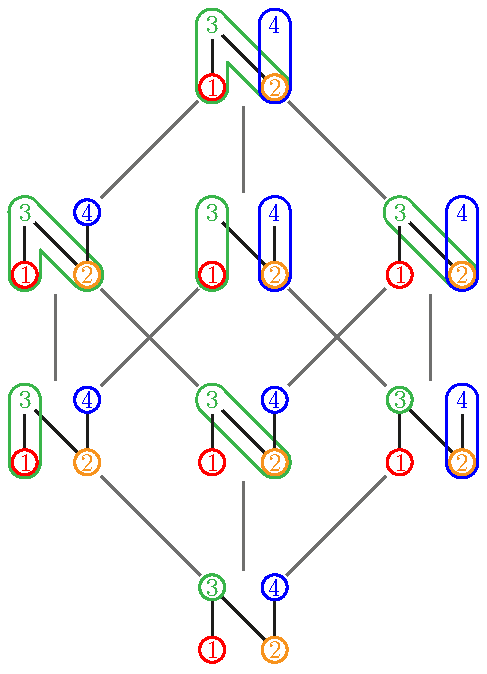
\includegraphics[scale=.8]{ornamentationsN} \qquad \raisebox{.5cm}{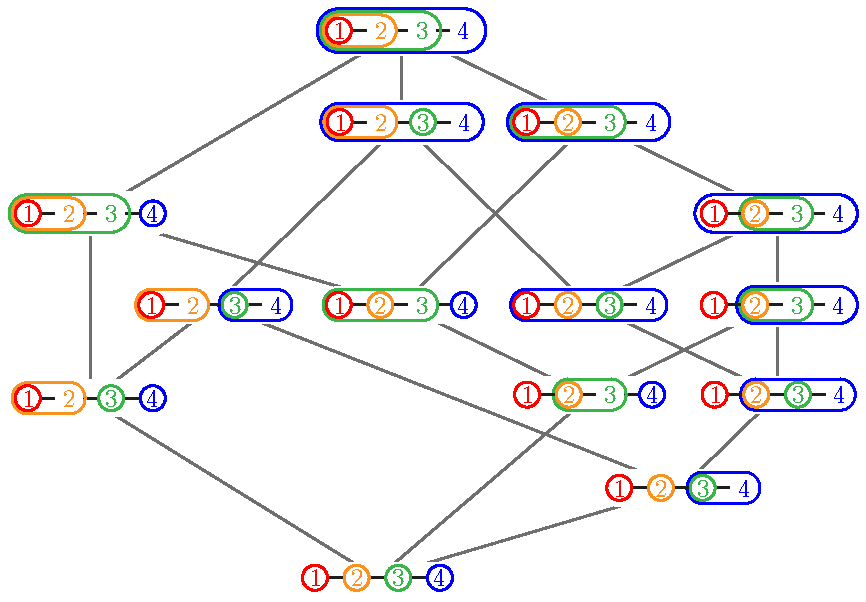
\includegraphics[scale=.8]{ornamentationsI}}}
	\caption{The ornamentation lattices~$\Orn(\Ngraph)$ and~$\Orn(\Igraph)$.}
	\label{fig:ornamentationsNI}
\end{figure}

\begin{figure}
	\centerline{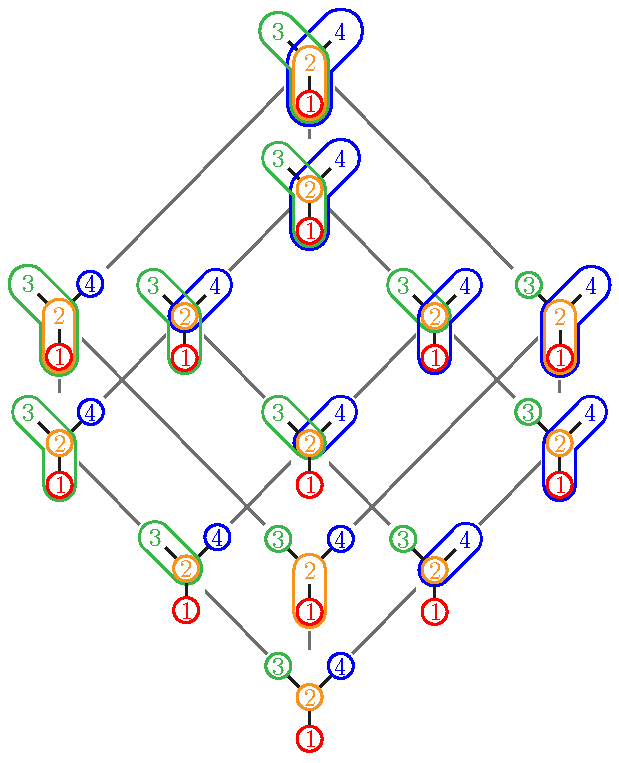
\includegraphics[scale=.8]{ornamentationsY} \qquad 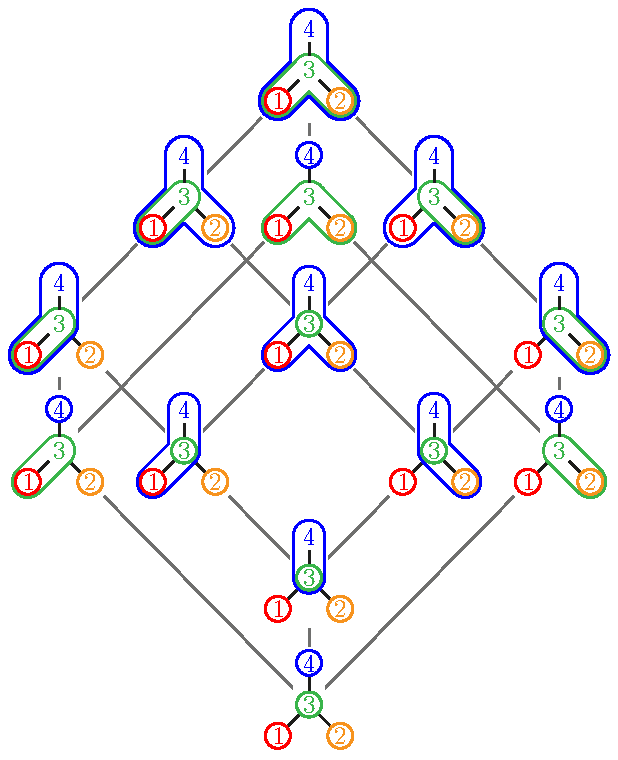
\includegraphics[scale=.8]{ornamentationsA}}
	\caption{The ornamentation lattices~$\Orn(\Ygraph)$ and~$\Orn(\Agraph)$.}
	\label{fig:ornamentationsAY}
\end{figure}

Throughout this section, we fix a directed graph~$D$ on a vertex set~$V$.
In all our pictures, $V = [n]$ and the edges are increasing (so we do not need to explicitly indicate the orientation).
%We will mostly work with a directed acyclic graph, and we represent it with edges going up in all pictures.
The following definition, first introduced for rooted trees in~\cite{} and extended to arbitrary directed graphs in~\cite{}, is illustrated in \cref{fig:ornamentationsNI,fig:ornamentationsAY,fig:ornamentationsX,fig:ornamentationsD}

\begin{definition}
An \defn{ornament} at a vertex $v$ of~$D$ is a subset~$U \subseteq V$ such that there is a path from any $u \in U$ to~$v$ in the directed subgraph of~$D$ induced by~$U$.
An \defn{ornamentation} of~$D$ is a map $O$ on $V$ which assigns an ornament~$O(v)$ at each vertex~$v \in V$ such that~$u \in O(v) \implies O(u) \subseteq O(v)$ for all~$u,v \in V$.
We denote by~$\Orn(v \in D)$ the set of ornaments at a vertex~$v$ of~$D$ and by~$\Orn(D)$ the set of ornamentations of~$D$.
\end{definition}

\begin{example}
We can define ornamentations by
\begin{itemize}
\item sending each vertex~$v \in V$ to the singleton~$\{v\}$, 
\item sending each vertex~$v \in V$ to the set~$U$ of vertices with a path to~$v$ in~$D$,
\item for any ornament~$U \in \Orn(v \in D)$, sending~$v$ to~$U$ and any other vertex~$u \in V \ssm \{v\}$ to the singleton~$\{u\}$.
\end{itemize}
\end{example}

\begin{lemma}
\label{lem:unionOrnaments}
\begin{enumerate}[(i)]
\item If~$U \in \Orn(u \in D)$ and~$U' \in \Orn(u' \in D)$ with~$u \in U'$, then~${U \cup U' \in \Orn(u' \in D)}$.
%\item If~$U$ is an ornament at a vertex~$u$ of~$D$ and~$U'$ is an ornament at a vertex~$u'$ of~$D$ and~$u \in U'$, then~$U \cup U'$ is an ornament of~$D$ at~$u'$.
\item If~$U,U' \in \Orn(v \in D)$, then~$U \cup U' \in \Orn(v \in D)$, while $U \cap U'$ is not necessarily~in~${\Orn(v \in D)}$.
%\item If~$U,U'$ are two ornaments at a vertex~$v$ of~$D$, then~$U \cup U'$ is also an ornament at~$v$, while $U \cap U'$ is not necessarily an ornament at~$v$.
\end{enumerate}
\end{lemma}

\begin{proof}
For Part~(i), let~$w \in U \cup U'$. If~$w \in U'$, then there is a path from~$w$ to~$u'$ in~$U'$, hence in~$U \cup U'$.
If~$w \in U$, then there is a path from~$w$ to~$u$ in~$U$ and a path from~$u$ to~$u'$ in~$U'$, hence a path from~$w$ to~$u'$ in~$U \cup U'$.
Part~(ii) is a specialization of Part~(i) to~$u = v$ and~$u' = v$.
\end{proof}

\begin{theorem}
\label{thm:Orn-meet_and_join}
The set~$\Orn(D)$ of ornamentations of~$D$ is a lattice under componentwise inclusion, meaning~$O_1 \le O_2$ if~$O_1(v) \subseteq O_2(v)$ for all~$v \in V$.
For any two ornamentations~$O_1$ and~$O_2$ of~$D$,
\begin{itemize}
\item $(O_1 \meet O_2)(v)$ is the inclusion maximal ornament at~$v$ contained in~$O_1(v) \cap O_2(v)$,
%\item the join~$O_1 \join O_2$ is the ornamentation of~$D$ where~$(O_1 \join O_2)(v) = \set{u \in V}{u \, R \, v}$ where $R$ is the transitive closure of~$u \in O_1(v) \cup O_2(v)$.
\item $(O_1 \join O_2)(v)$ is the inclusion minimal subset~$U$ of~$V$ containing~$v$ and such that~$u \in U$ implies~$O_1(u) \cup O_2(u) \subseteq U$.
\end{itemize}
\end{theorem}

\begin{proof}
%Given two ornamentations~$O_1$ and~$O_2$ of~$D$, let~$O_\meet$ and $O_\join$ be the maps on~$V$ defined by 
%\begin{itemize}
%\item $O_\meet(v)$ is the inclusion maximal ornament at~$v$ contained in~$O_1(v) \cap O_2(v)$,
%%\item $O_\join(v) = \set{u \in V}{u \, R \, v}$ where $R$ is the transitive closure of~$u \in O_1(v) \cup O_2(v)$.
%\item $O_\join(v)$ is the inclusion minimal subset~$U$ of~$V$ containing~$v$ and such that~$u \in U$ implies~$O_1(u) \cup O_2(u) \subseteq U$.
%\end{itemize}
%
Given two ornamentations~$O_1$ and~$O_2$ of~$D$, consider the map~$O_\meet$ on~$V$ where $O_\meet(v)$ is the inclusion maximal ornament at~$v$ contained in~$O_1(v) \cap O_2(v)$.
Note that $O_\meet(v)$ is well defined by \cref{lem:unionOrnaments}, and that~$O_\meet(v) \in \Orn(v \in D)$ for any~$v \in V$ by definition.
Consider now~$u,v \in V$ such that~$u \in O_\meet(v)$.
Since~$O_\meet(u) \in \Orn(u \in D)$ and~$O_\meet(v) \in \Orn(v \in D)$ with~${u \in O_\meet(v)}$, \cref{lem:unionOrnaments} gives~$O_\meet(u) \cup O_\meet(v) \in \Orn(v \in D)$.
As~$u \in O_\meet(v) \subseteq O_1(v) \cap O_2(v)$ and~$O_1$ and~$O_2$ are ornamentations of~$D$, we have~$O_1(u) \subseteq O_1(v)$ and~$O_2(u) \subseteq O_2(v)$, so that~$O_\meet(u) \subseteq O_1(u) \cap O_2(u) \subseteq O_1(v) \cap O_2(v)$, hence~$O_\meet(u) \cup O_\meet(v) \subseteq O_1(v) \cap O_2(v)$.
By maximality of~$O_\meet(v)$, we conclude that $O_\meet(u) \cup O_\meet(v) \subseteq O_\meet(v)$, so that~$O_\meet(u) \subseteq O_\meet(v)$.
We conclude that~$O_\meet$ is an ornamentation of~$D$.
Moreover, $O_\meet$ is clearly the meet of~$O_1$ and~$O_2$ in componentwise inclusion.

Given two ornamentations~$O_1$ and~$O_2$ of~$D$, consider now the map~$O_\join$ on~$V$ where~$O_\join(v)$ is the inclusion minimal subset~$U$ of~$V$ containing~$v$ and such that~$u \in U$ implies~$O_1(u) \cup O_2(u) \subseteq U$.
Note that~$O_\join(v)$ is well defined as it can be constructed by induction, starting from~$U = \{v\}$ and adding inductively~$O_1(u) \cup O_2(u)$ for all~$u \in U$ until it stabilizes.
Since~$O_1(u) \cup O_2(u) \in \Orn(u \in D)$ by \cref{lem:unionOrnaments}, this inductive construction maintains the invariant that there is a path from~$u$ to~$v$ in~$U$ for any~$u \in U$.
Hence, we obtain that~$O_\join(v) \in \Orn(v \in D)$ for any~$v \in V$.
Consider now~$u,v \in V$ such that~$u \in O_\join(v)$.
Since~$u \in O_\join(v)$ and~$w \in O_\join(v)$ implies~$O_1(w) \cup O_2(w) \subseteq O_\join(v)$, we obtain that~$O_\join(u) \subseteq O_\join(v)$ by minimality of~$O_\join(u)$.
We conclude that~$O_\join$ is an ornamentation of~$D$.
Moreover, $O_\join$ is clearly the join of~$O_1$ and~$O_2$ in componentwise inclusion.
\end{proof}

\begin{example}
The ornamentation lattice of the graph with a single edge is a $2$-elements chain.
The ornamentation lattice of a graph with no path of length $2$ is a boolean lattice (see \eg \cref{fig:ornamentationsNI}\,(left) and \cref{fig:ornamentationsT}).
%In general, the ornamentation lattice~$\Orn(D \sqcup D')$ of the disjoint union of two directed graphs~$D$ and~$D'$ is the Cartesian product~$\Orn(D) \times \Orn(D')$ of the ornamentation lattices of~$D$ and~$D'$
\end{example}

\begin{example}
The ornamentation lattice of a $n$-elements path is isomorphic to the Tamari lattice on binary trees with $n$ nodes (see \eg \cref{fig:ornamentationsNI}\,(right)).
The isomorphism is obtained trough tubings (or equivalently bracket vectors).
\end{example}

\begin{remark}
\label{rem:posetPropertiesOrnamentations}
A few poset properties of the ornamentations lattice~$\Orn(D)$:
\begin{itemize}
\item The minimal ornamentation sends each vertex~$v \in V$ to the singleton~$\{v\}$, and the maximal ornamentation sends each vertex~$v \in V$ to the set~$U$ of vertices with a path to~$v$ in~$D$.
\item Two ornamentations~$O_1$ and~$O_2$ of~$D$ form a cover relation if and only if there is~$u, v \in V$ such that~$u \notin O_1(v)$ and~$O_2(v) = O_1(u) \cup O_1(v)$, while~$O_1(w) = O_2(w)$ for all~$w \in V \ssm \{v\}$.
\item For any~$U \subseteq V$, the ornamentation lattice of the subgraph~$D_U$ of~$D$ induced by~$U$ is an interval of the ornamentation lattice of~$D$ (namely, the bottom interval below the ornamentation of~$D$ where~$O(u)$ is the set of vertices of~$U$ with a path to~$u$ in~$U$ for all~$u \in U$, while~$O(v)$ is the singleton~$\{v\}$ for all~$v \in V \ssm U$).
\end{itemize}
\end{remark}

\begin{remark}
A few lattice properties of the ornamentation lattice~$\Orn(D)$:
\begin{itemize}
\item The join irreducible ornamentations of~$D$ are precisely the ornamentations~$\Orn_P$ described in \cref{rem:posetPropertiesOrnamentations} for the directed paths~$P$ in~$D$ which admit no shortcut in~$D$. (The meet irreducible ornamentations are more complicated to describe.)
\item $\Orn(D)$ is distributive if and only if~$D$ contains no path of length~$2$ (in which case, $\Orn(D)$ is actually a boolean lattice).
\item $\Orn(D)$ is semidistributive if and only if~$D$ is a directed tree.
\end{itemize}
\end{remark}

\begin{figure}[p]
	\centerline{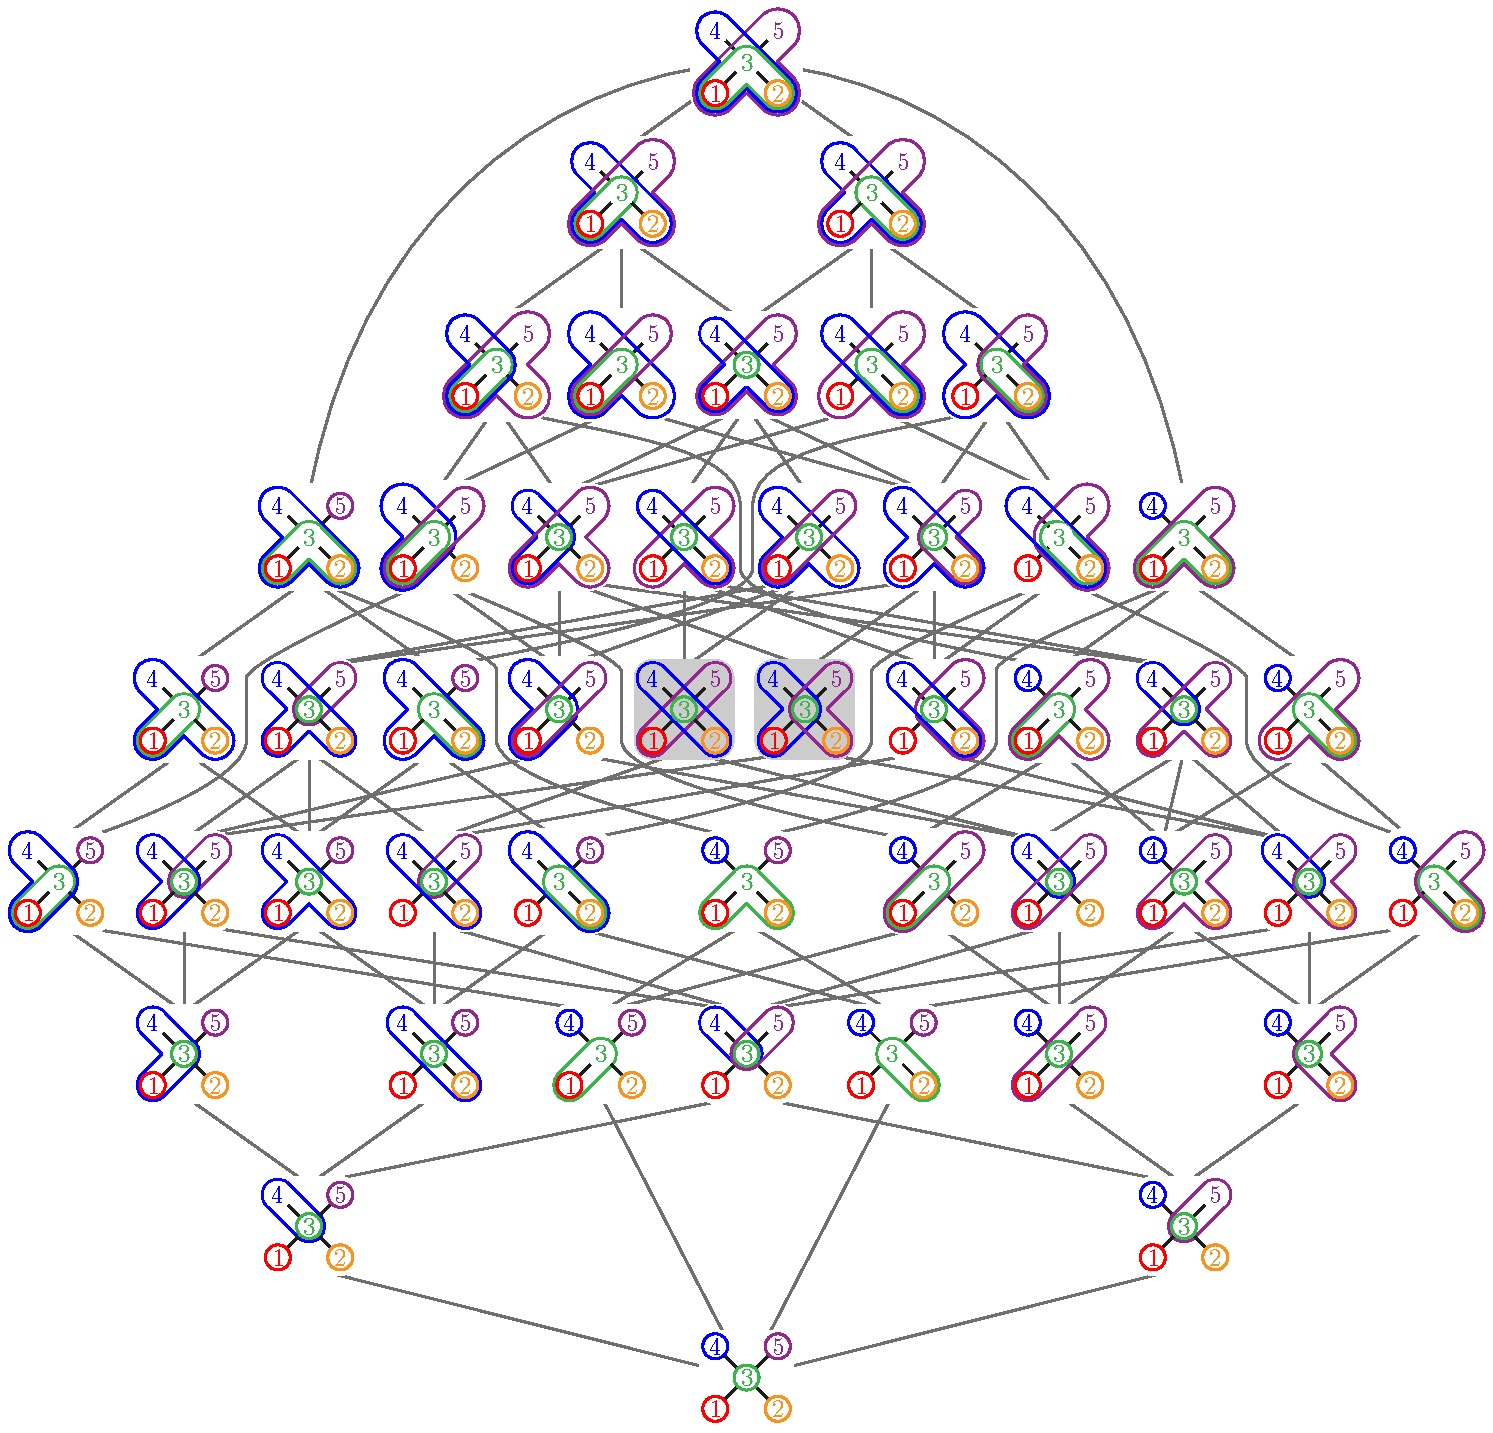
\includegraphics[scale=.8]{ornamentationsX}}
	\caption{The ornamentation lattice~$\Orn(\Xgraph)$ of the directed graph~$\Xgraph$.}
	\label{fig:ornamentationsX}
\end{figure}

\begin{figure}
	\centerline{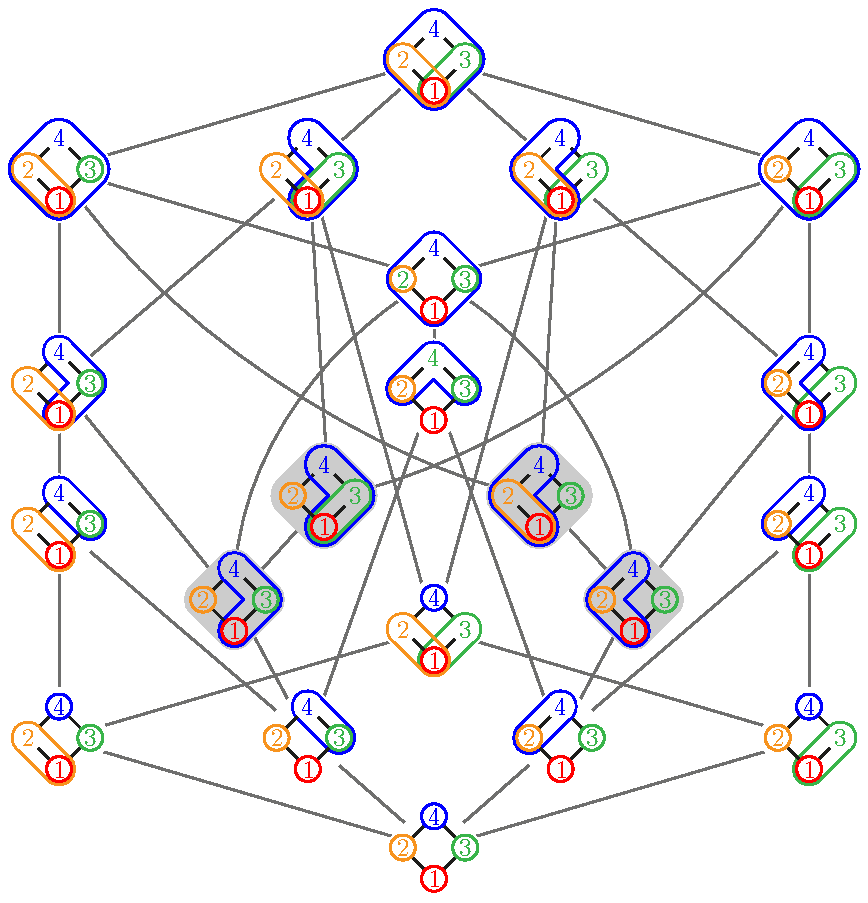
\includegraphics[scale=.8]{ornamentationsD}}
	\caption{The ornamentation lattice~$\Orn(\Dgraph)$ of the directed graph~$\Dgraph$.}
	\label{fig:ornamentationsD}
\end{figure}

\begin{figure}
	\centerline{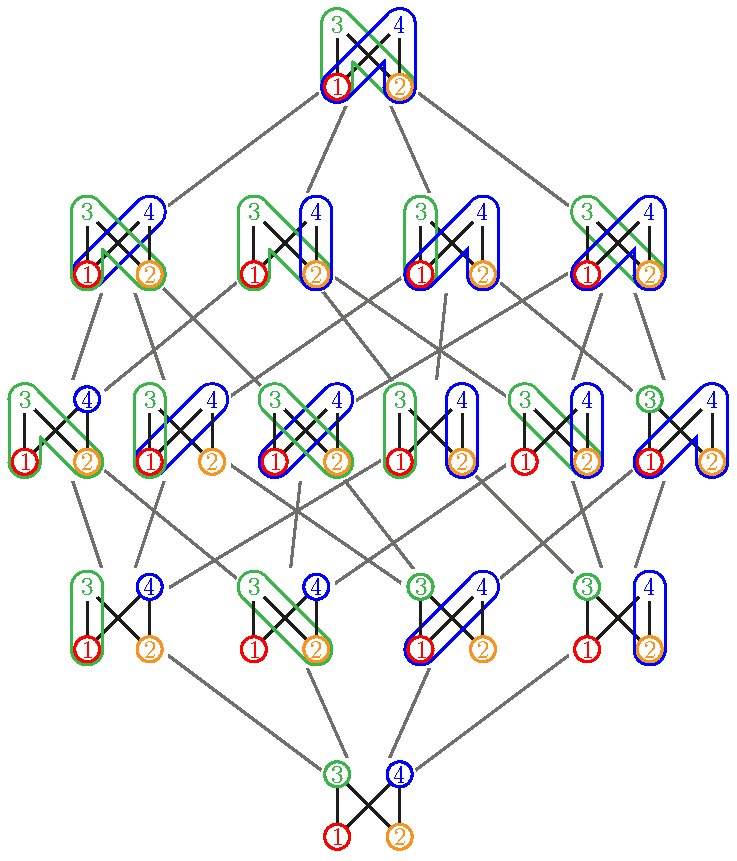
\includegraphics[scale=.8]{ornamentationsT}}
	\caption{The ornamentation lattice~$\Orn(\Tgraph)$ of the directed graph~$\Tgraph$.}
	\label{fig:ornamentationsT}
\end{figure}

Answering a question opened in~\cite{DelfantSack}, we will prove the following statement in the next section.

\begin{theorem}
The Hasse diagram of the ornamentation lattice of a rooted tree is isomorphic to the skeleton of a polytope oriented in a linear direction. 
\end{theorem}

This question remains open beyond the case of rooted trees.
We state it as a conjecture.

\begin{conjecture}
The Hasse diagram of the ornamentation lattice of any directed graph is isomorphic to the skeleton of a polytope oriented in a linear direction. 
\end{conjecture}

%%%%%%%%%%%%%%%%%%%%%%%%%%%%%%%%%%%%%%
%%%%%%%%%%%%%%%%%%%%%%%%%%%%%%%%%%%%%%
%%%%%%%%%%%%%%%%%%%%%%%%%%%%%%%%%%%%%%

\section{From reorientations to ornamentations}
\label{sec:reorientations}

\begin{definition}
A \defn{reorientation}~$R$ of a directed graph~$E$ is a directed graph obtained from~$E$ by reversing a subset~$\rev(R)$ of arrows of~$E$.
The \defn{reorientation lattice}~$\Reori(E)$ of~$E$ is the boolean lattice of reorientations of~$E$, ordered by inclusion of subsets of reversed arrows, meaning $R_1 \le R_2$ if ${\rev(R_1) \subseteq \rev(R_2)}$.
\end{definition}

In this paper, we actually need to consider the reorientation lattice~$\Reori(\tc(D))$ of the transitive closure~$\tc(D)$ of the directed graph~$D$.
Recall that, for all~$u,v \in V$, the transitive closure~$\tc(D)$ has an arc~$(u,v)$ if and only if~$D$ has a directed path from~$u$ to~$v$.
There is a natural surjection from the reorientation lattice~$\Reori(\tc(D))$ to the ornamentation lattice~$\Orn(D)$.

\begin{definition}
\label{def:Reori2Orn}
For a reorientation~$R$ of~$\tc(D)$, we define a map~$\orn{R}$ on~$V$ which associates to each vertex~$v \in V$ the inclusion maximal ornament of~$D$ at~$v$ contained in the subset of vertices~$u \in V$ with a directed path to~$v$ in $\rev(R)$.
\end{definition}

\begin{lemma}
\label{lem:Reori2Orn1}
For any reorientation~$R$ of~$\tc(D)$, the map~$\orn{R}$ is an ornamentation of~$D$.
\end{lemma}

\begin{proof}
By definition, $\orn{R}(v) \in \Orn(v \in D)$ for all~$v \in V$.
Consider now~$u,v \in V$ such that~$u \in \orn{R}(v)$.
Since~$\orn{R}(u) \in \Orn(u \in D)$ and~$\orn{R}(v) \in \Orn(v \in D)$ with~${u \in \orn{R}(v)}$, \cref{lem:unionOrnaments} gives~$\orn{R}(u) \cup \orn{R}(v) \in \Orn(v \in D)$.
Moreover, by path concatenation, there is a path from any vertex of~$\orn{R}(u) \cup \orn{R}(v)$ to~$v$ in~$\rev(R)$.
By maximality of~$\orn{R}(v)$, we conclude that~$\orn{R}(u) \subseteq \orn{R}(v)$, so that~$\orn{R}(u) \subseteq \orn{R}(v)$.
\end{proof}

\begin{lemma}
\label{lem:Reori2Orn2}
The map~$R \mapsto \orn{R}$ is order-preserving (meaning that~$R_1 \le R_2 \implies \orn{R_1} \le \orn{R_2}$).
\end{lemma}

\begin{proof}
If~$R_1 \le R_2$, then $\rev(R_1) \subseteq \rev(R_2)$, hence any path in~$\rev(R_1)$ is a path in~$\rev(R_2)$, so that~$\orn{R_1}(v) \subseteq \orn{R_2}(v)$ for any~$v \in V$, hence~$\orn{R_1} \le \orn{R_2}$.
\end{proof}

\begin{definition}
For an ornamentation~$O$ of~$D$, we define a reorientation~$\reori{O}$ of~$\tc(D)$ where for each~$(u,v) \in \tc(D)$, we have~$(u,v) \in \rev(\reori{O})$ if and only if~$u \in O(v)$.
\vincent{This map is not compatible with acyclicity later...}
\end{definition}

\begin{lemma}
\label{lem:Orn2Reori1}
The map~$O \mapsto \reori{O}$ is order-preserving.
\end{lemma}

\begin{proof}
If~$O_1 \le O_2$, then $O_1(v) \subseteq O_2(v)$ for all~$v \in V$, thus~$\rev(\reori{O_1}) \subseteq \rev(\reori{O_2})$, hence~${\reori{O_1} \le \reori{O_2}}$.
\end{proof}

\begin{lemma}
\label{lem:Orn2Reori2}
The map~$O \mapsto \reori{O}$ is a section of the map~$R \mapsto \orn{R}$.
\end{lemma}

\begin{proof}
Let~$u,v \in V$ such that there is a path from~$u$ to~$v$ in~$\rev(\reori{O})$.
Let~$u = w_0, w_1, \dots, w_p = v$ denote the vertices along this path.
We have~$(w_{i-1},w_i) \in \rev(\reori{O})$ hence~$w_{i-1} \in O(w_i)$ for each~$1 \le i \le p$.
Since~$O$ is an ornamentation, an immediate induction shows that~$w_i \in O(v)$ for all~$0 \le i \le p$.
We conclude that $u \in O(v)$ if and only if there is a path from~$u$ to~$v$ in~$\rev(\reori{O})$.
Since~$O(v)$ is an ornament of~$D$ at~$v$, we conclude that~$\orn{\reori{O}}(v) = O(v)$.
\end{proof}

To sum up, we obtained the following statement.

\begin{proposition}
The map~$R \mapsto \orn{R}$ is an order-preserving surjection from the reorientation lattice~$\Reori(\tc(D))$ to the ornamentation lattice~$\Orn(D)$.
\end{proposition}

Unfortunately, this surjection does not preserve the lattice structure, as illustrated by the following example.

\begin{example}
\vincent{todo}
\end{example}

To correct this default, we restrict our attention to transitively closed reorientations.

\begin{definition}
A reorientation~$R$ of~$\tc(D)$ is \defn{transitively closed} if~$\rev(R)$ is transitively closed %, that is~$(u,v), (v,w) \in \rev(R)$ implies $(u,w) \in \rev(R)$.
and \defn{transitively coclosed} if the complement~$\tc(D) \ssm \rev(R)$ is transitively closed.
We denote by~$\Rcl(\tc(D))$ and $\Rco(\tc(D))$ the sets of transitively closed and transitively coclosed reorientations of $\tc(D)$ respectively.
\end{definition}

\begin{lemma}
\label{lem:rcl-subsemilattice}
$\Rcl(\tc(D))$ (resp.~$\Rco(\tc(D))$) induces a meet (resp.~join) subsemilattice of~$\Reori(\tc(D))$, which is a lattice.
\end{lemma}

\begin{proof}
As the intersection of two transitively closed relations is transitively closed, $R, R' \in \Rcl(\tc(D))$ implies $R \meet R' \in \Rcl(\tc(D))$.
As~$\tc(D)$ is transitively closed, the maximal reorientation of~$\tc(D)$ is transitively closed, so that $\Rcl(\tc(D))$ is a bounded meet semilattice, hence a lattice.
The proof for~$\Rco(\tc(D))$ is symmetric.
\end{proof}

\begin{lemma}
For any ornamentation~$O$ of~$D$, the reorientation~$\reori{O}$ is transitively closed. Hence, the map~$R \mapsto \orn{R}$ restricts to a surjection from the transitively closed reorientation lattice~$\Rcl(\tc(D))$ to the ornamentation lattice~$\Orn(D)$.
\end{lemma}

\begin{proof}
Let~$u,v,w \in V$ such that~$(u,v), (v,w) \in \rev(\reori{O})$.
Then~$u \in O(v)$ and~$v \in O(w)$, so that~$u \in O(w)$ since~$O$ is an ornamentation.
Hence~$(u,w) \in \rev(\reori{O})$.
\end{proof}

\begin{proposition}
The map~$R \mapsto \orn{R}$ is a meet semilattice morphism from the transitively closed reorientation lattice~$\Rcl(\tc(D))$ to the ornamentation lattice~$\Orn(D)$.
\end{proposition}

\begin{proof}
\vincent{Todo. See notes of Jose and Antoine.}
\jose{I have added the details, feel free to rewrite if necessary.}
Let $R$ and $R'$ be two transitively closed reorientations of $\tc(D)$, and $O_\meet = \orn{R} \meet \orn{R'}$.
We want to show that $O_\meet = \orn{R \meet R'}$.

Let $u \in O_\meet(v)$.
Then, there exists a path from $u$ to $v$ in $O_\meet(v) \subseteq \orn{R}(v) \cap \orn{R'}(v)$.
Let~$u = w_0, w_1, \dots, w_p = v$ denote the vertices along this path.
By definition of $\orn{R}$ and $\orn{R'}$, there is a path from each $w_i$ to $v$ in both $\rev(R)$ and $\rev(R')$.
Since $R$ and $R'$ are transitively closed, each arrow $(w_i,v)$ of $\tc(D)$ is in both $\rev(R)$ and $\rev(R')$;
and therefore in $\rev(R \meet R') = \rev(R) \cap \rev(R')$ (\cref{lem:rcl-subsemilattice}).
So, $\{u = w_0, w_1, \dots, w_p = v\} \in \Orn(v \in D)$ and each $w_i$ has a directed path to $v$ in $\rev(R) \cap \rev(R')$.
By maximality of $\orn{R \meet R'}(v)$, we deduce $u \in \orn{R \meet R'}(v)$.
Thus, we have shown that $O_\meet \leq \orn{R \meet R'}$.

Now let $u \in \orn{R \meet R'}(v)$ and
let $u = w_0, w_1, \dots, w_p = v$ denote the vertices along a path from $u$ to $v$ in $\orn{R \meet R'}(v)$.
Thus, each arrow $(w_i,v)$ of $\tc(D)$ is in $\rev(R \meet R') = \rev(R) \cap \rev(R')$,
showing that this same path is contained in both $\orn{R}(v)$ and $\orn{R'}(v)$.
By \cref{thm:Orn-meet_and_join}, $\{u = w_0, w_1, \dots, w_p = v\} \subseteq O_\meet(v)$.
We have shown that $O_\meet \geq \orn{R \meet R'}$, and therefore they are equal.
\end{proof}

%%%%%%%%%%%%%%%%%%%%%%%%%%%%%%%%%%%%%%
%%%%%%%%%%%%%%%%%%%%%%%%%%%%%%%%%%%%%%
%%%%%%%%%%%%%%%%%%%%%%%%%%%%%%%%%%%%%%

\section{From sourcings to ornamentations}
\label{sec:sourcings}

We now assume that~$V$ is totally ordered, say that~$V = [n]$ with the natural order.
%We now assume that~$D$ is an increasing graph on~$V = [n]$.

\begin{definition}
A \defn{sourcing}~$S$ of a hypergraph~$\HH$ on~$V$ is a map~$S : \HH \to V$ such that~$S(H) \in H$ for all hyperedges~$H \in \HH$.
We denote by~$\rev(S)$ the pairs~$(u,v) \in V^2$ with~$u < v$ and such that there is~$H \in \HH$ with~$u \in H$ and~$v = S(H)$,
The \defn{sourcing lattice}~$\Sour(\HH)$ is the lattice of sourcings of~$\HH$ ordered componentwise, meaning~$S_1 \le S_2$ if~$S_1(H) \le S_2(H)$ for all~$H \in \HH$.
In other words, $\Sour(\HH)$ is the Cartesian product of the subchains of~$V$ induced by the hyperedges~$\HH$.
\end{definition}

%In this paper, we will consider sourcings of the interval hypergraph of~$D$.
%
%\begin{definition}
%Let~$D$ be a directed graph on~$V$.
%For~$u,v \in V$, the \defn{interval}~$[u,v]$ is the union of all directed paths from~$u$ to~$v$.
%The \defn{interval hypergraph} of~$D$ is the collection~$\II$(D) of non-empty intervals~$[u,v]$ for all~$u,v \in V$.
%\end{definition}

We now assume that~$D$ is an increasing graph on~$V = [n]$, and we consider sourcings of the path hypergraph of~$D$.

\begin{definition}
The \defn{path hypergraph} of a directed graph~$D$ is the collection~$\PP$(D) of vertex sets of directed paths in~$D$.
\end{definition}

We first observe that any sourcing~$S$ of~$\PP(D)$ can be lifted to a reorientation~$\reori{S}$ of~$\tc(D)$

\begin{definition}
\label{def:Sour2Reori}
For a sourcing~$S$ of~$\PP(D)$, we denote by~$\reori{S}$ the reorientation of~$\tc(D)$ defined by~$\rev(\reori{S}) = \rev(S)$.
\vincent{This map is not compatible with acyclicity later...}
\end{definition}

\begin{lemma}
\label{lem:Sour2Reori}
The map~$S \mapsto \reori{S}$ is order-preserving.
\end{lemma}

\begin{proof}
If~$S_1 \le S_2$, then $\rev(S_1) \subseteq \rev(S_2)$, hence $\rev(\reori{S_1}) \subseteq \rev(\reori{S_2})$, hence~$\reori{S_1} \le \reori{S_2}$.
\end{proof}

In contrast, not all reorientations of~$\tc(D)$ can be projected to a sourcing of~$\PP(D)$, because reorientations might have cycles inside paths of~$D$.
We will fix this problem by restricting to acyclic reorientations and acyclic sourcings in \cref{sec:acyclic}.
At the moment, we thus need define a map from all sourcings of~$\PP(D)$ to all ornamentations of~$D$.

\begin{definition}
\label{def:Sourc2Orn}
For a sourcing~$S$ of~$\PP(D)$, we define a map~$\orn{S}$ on~$V$ which associates to each vertex~$v \in V$ the inclusion maximal ornament of~$D$ at~$v$ contained in the subset of vertices~$u \in V$ with a directed path to~$v$ in $\rev(S)$. % such that there is~$P_0, \dots, P_k \in \PP(D)$ with~$u \in P_0 \ssm \{S(P_0)\}$, $v = S(P_k)$, and~$S(P_{i-1}) \in P_i \ssm \{S(P_i)\}$ for~all~$i \in [k]$.
\end{definition}

\begin{lemma}
\label{lem:Sour2Orn2}
For any sourcing~$S$ of~$\PP(D)$, the map~$\orn{S}$ is an ornamentation of~$D$.
\end{lemma}

\begin{proof}
The proof is identical to that of~\cref{lem:Reori2Orn1}.
In fact, it also follows from~\cref{lem:Reori2Orn1} since~$\orn{S} = \orn{\reori{S}}$.
\end{proof}

\begin{lemma}
\label{lem:Sour2Orn2}
The map~$S \mapsto \orn{S}$ is order-preserving.
\end{lemma}

\begin{proof}
The proof is identical to that of~\cref{lem:Reori2Orn2}.
In fact, it also follows from~\cref{lem:Reori2Orn2,lem:Sour2Reori} since~$\orn{S} = \orn{\reori{S}}$.
%If~$S_1 \le S_2$, then $\rev(S_1) \subseteq \rev(S_2)$, hence any path in~$\rev(S_1)$ is a path in~$\rev(S_2)$, so that~$\orn{S_1}(v) \subseteq \orn{S_2}(v)$ for any~$v \in V$, hence~$\orn{S_1} \le \orn{S_2}$.
\end{proof}

\begin{definition}
For an ornamentation~$O$ of~$D$, we define a sourcing~$\sour{O}$ of~$\PP(D)$ where the source~$\sour{O}(P)$ for a path~$P$ from~$u$ to~$v$ in~$D$ is the maximal~$w \in P$ such that~$u \in O(w)$.
\end{definition}

\begin{lemma}
\label{lem:Orn2Sour1}
The map~$O \mapsto \sour{O}$ is order-preserving.
\end{lemma}

\begin{proof}
Assume that~$O_1 \le O_2$, so that~$O_1(v) \subseteq O_2(v)$ for all~$v \in V$.
Consider any path~$P$ from~$u$ to~$v$, and let~$w \eqdef \sour{O_1}(P)$.
Then we have~$u \in O_1(w) \subseteq O_2(w)$, so that~$\sour{O_2}(u) \ge w$ by definition.
Therefore, $\sour{O_1}(P) \le \sour{O_2}(P)$ for any path~$P \in \PP(D)$, hence~${\sour{O_1} \le \sour{O_2}}$.
\end{proof}

\begin{lemma}
\label{lem:Orn2Sour2}
The map~$O \mapsto \sour{O}$ is a section of the map~$S \mapsto \orn{S}$.
\end{lemma}

\begin{proof}
Let~$u,v \in V$.
If~$u \in O(v)$, then there is a path~$P$ from~$u$ to~$v$ in~$O(v)$, hence~$(u,v) \in \rev(\sour{O})$.
Assume that there is a path from~$u$ to~$v$ in~$\rev(\sour{O})$.
Let~$u = w_0 \le w_1 \le \dots \le w_p = v$ denote the vertices along this path.
For each $1 \le i \le p$, there is a path~$P_i$ in~$D$ such that~$w_{i-1} \in P_i$ and~$w_i = \sour{O}(P_i)$, hence~$w_{i-1} \in O(w_i)$.
Since~$O$ is an ornamentation, an immediate induction shows that~$w_i \in O(v)$ for all~$0 \le i \le p$.
We conclude that $u \in O(v)$ if and only if there is a path from~$u$ to~$v$ in~$\rev(\sour{O})$.
Since~$O(v)$ is an ornament of~$D$ at~$v$, we conclude that~$\orn{\sour{O}}(v) = O(v)$.
\end{proof}

To sum up, we obtained the following statement.

\begin{proposition}
The map~$S \mapsto \orn{S}$ is an order-preserving surjection from the sourcing lattice~$\Sour(\PP(D))$ to the ornamentation lattice~$\Orn(D)$.
\end{proposition}

\begin{remark}
The map~$S \mapsto \orn{S}$ is obviously not injective.
For instance, $\orn{S}$ is the maximal ornamentation of~$D$ for any sourcing~$S$ of~$\PP(D)$ such that~$S(\{u,v\}) = v$ for each edge~$(u,v)$ of~$D$.
In contrast, we will see in \cref{sec:acyclic} that~$S \mapsto \orn{S}$ is injective on acyclic sourcings of~$\PP(D)$.
\end{remark}

\vincent{We can play the same game with transitively closed sourcings~$S$, meaning for which $\rev(S)$ is transitively closed...}


%%%%%%%%%%%%%%%%%%%%%%%%%%%%%%%%%%%%%%
%%%%%%%%%%%%%%%%%%%%%%%%%%%%%%%%%%%%%%
%%%%%%%%%%%%%%%%%%%%%%%%%%%%%%%%%%%%%%

\section{Acyclic reorientations, acyclic sourcings, and acyclic ornamentations}
\label{sec:acyclic}

We now focus our attention on the acyclic situation.
We assume here that~$D$ is an increasing graph on~$V = [n]$, meaning that $i < j$ for any arc~$(i,j)$ of~$D$, in particular~$D$ is acyclic.
We then consider the acyclic reorientation poset~$\AReori(\tc(D))$, the acyclic sourcing poset~$\ASour(\PP(D))$, and the acyclic ornamentation poset~$\AOrn(D)$, and define natural surjective poset morphisms:
\[
\begin{array}{rcccccl}
	\fS_n & \surjection & \AReori(\tc(D)) & \surjection & \ASour(\PP(D)) & \bijection & \AOrn(D) \\
	\pi & \longmapsto & \areori{\pi} \qquad R & \longmapsto & \asour{R} \qquad S & \longmapsto & \aorn{S}
\end{array}
\]

\subsection{Acyclic reorientations}

Acyclic reorientations of directed acyclic graphs is a classical subject, see for instance~\cite{Pilaud-acyclicReorientationLattices}.

\begin{definition}
A reorientation of a directed graph~$E$ is \defn{acyclic} if it contains no directed cycle.
The \defn{acyclic reorientation poset}~$\AReori(E)$ is the subposet of the reorientation lattice~$\Reori(E)$ induced by acyclic reorientations.
\end{definition}

\begin{remark}
Let us recall the polytopal interpretation of the acyclic reorientation poset of~$E$.
Denote by~$(\b{e}_i)_{i \in [n]}$ the standard basis of~$\R^n$.
The \defn{graphical zonotope} of~$E$ is the Minkowski sum~$\simplex_E \eqdef \sum_{(u,v) \in E} \simplex_{uv}$, where~$\simplex_{uv}$ is the segment with endpoints~$\b{e}_u$ and~$\b{e}_v$.
The face lattice of~$\simplex_E$ is described by ordered partitions of~$E$.
In particular, the graph of~$\simplex_E$, oriented in the direction~$\b{\omega} \eqdef (n, n-1, \dots, 2, 1) - (1, 2, \dots, n-1, n) = (n-1, n-3, \dots, 3-n, 1-n)$, is isomorphic to the Hasse diagram of the acyclic reorientation poset~$\AReori(E)$.
\end{remark}

Note that the acyclic reorientation poset~$\AReori(E)$ is not always a lattice.
The lattice theory of acyclic reorientation posets was studied in details in~\cite{Pilaud-acyclicReorientationLattices}.
For our purposes, we will only need the following characterization.

\begin{proposition}[{\cite[Thm.~1]{Pilaud-acyclicReorientationLattices}}]
\label{prop:acyclicReorientationLattices}
The acyclic reorientation poset~$\AReori(E)$ is a lattice if and only if the transitive reduction of any induced subgraph of~$E$ is a forest.
\end{proposition}

We now recall the standard map from permutations to acyclic orientations.

\begin{definition}
For a permutation~$\pi$ of~$[n]$, we denote by~$\areori{\pi}$ the reorientation of~$\tc(D)$ where $(u,v) \in \tc(D)$ is reoriented in~$\areori{\pi}$ if~$\pi^{-1}(u) > \pi^{-1}(v)$.
\end{definition}

\begin{proposition}
The map~$\pi \mapsto \areori{\pi}$ is an order-preserving surjection from the weak order~$\fS_n$ to the acyclic reorientation poset~$\AReori(\tc(D))$.
\end{proposition}

\begin{proof}
Recall that the weak order on~$\fS_n$ is defined by the inclusion of inversion sets, where the inversion set of~$\pi \in \fS_n$ is~$\inv(\pi) \eqdef \set{(u,v)}{u < v \text{ and } \pi^{-1}(u) > \pi^{-1}(v)}$.
By definition, we have~$\rev(\areori{\pi}) = \inv(\pi) \cap \tc(D)$, hence~$\pi \mapsto \areori{\pi}$ is order-preserving.
It is surjective since the fiber of any reorientation~$R$ is the set of linear extensions of~$R$, which is non-empty when~$R$ is acyclic.
\end{proof}

\subsection{Acyclic sourcings}

Acyclic sourcings of hypergraphs were introduced in~\cite{BenedettiBergeronMachacek,BergeronPilaud} as combinatorial models for the vertex sets of hypergraphic polytopes.

\begin{definition}
A sourcing~$S$ of a hypergraph~$\HH$ is \defn{acyclic} if there is no distinct~$H_0, \dots, H_k \in \HH$ such that~$S(H_{i-1}) \in H_i \ssm \{S(H_i)\}$ for all~$i \in [k]$ and~$S(H_k) \in H_0 \ssm \{S(H_0)\}$.
The \defn{acyclic sourcing poset}~$\ASour(\HH)$ is the subposet of the sourcing lattice~$\Sour(\HH)$ induced by acyclic sourcings.
\end{definition}

\begin{remark}
Let us recall the polytopal interpretation of the acyclic sourcing poset of a hypergraph~$\HH$.
We still denote by~$(\b{e}_i)_{i \in [n]}$ the standard basis of~$\R^n$.
The \defn{hypergraphic polytope} of~$\HH$ is the Minkowski sum
\(
\simplex_\HH \eqdef \sum_{H\in \HH} \simplex_H\,,
\)
where $\simplex_H$ is the simplex given by the convex hull of the points $\b{e}_h$ for~$h \in H$.
The face lattice of~$\simplex_\HH$ was described combinatorially in terms of acyclic orientations of~$\HH$ in~\cite{BenedettiBergeronMachacek}.
In particular, the transitive closure of the graph of~$\simplex_\HH$, oriented in the direction~$\b{\omega}$, is isomorphic to the acyclic sourcing poset~$\ASour(\HH)$.
Note that the graph of~$\simplex_\HH$, oriented in the direction~$\b{\omega}$, is not always transitively reduced, hence not always isomorphic to the Hasse diagram of the acyclic sourcing poset~$\ASour(\HH)$.
\end{remark}

Note that the acyclic sourcing poset of~$\HH$ is not always a lattice.
Characterizing the hypergraphs whose acyclic sourcing poset is a lattice seems a difficult question in general.
Such characterizations exist for specific families of hypergraphs, notably for graphs~\cite{Pilaud-acyclicReorientationLattices} (see \cref{prop:acyclicReorientationLattices}), interval hypergraphs~\cite{BergeronPilaud}, and (partially for) graph associahedra~\cite{BarnardMcConville}.
We will further study this question for subhypergraphs of the path hypergraph of directed trees in \cref{sec:intreevalHypergraphicPosets}.

We have observed in \cref{sec:sourcings} that there is no natural surjection from all reorientations of~$\tc(D)$ to all sourcings of~$\PP(D)$.
We now recall that there is such a surjection when focussing on acyclic reorientations and acyclic sourcings.

\begin{definition}
For an acyclic reorientation~$R$ of~$\tc(D)$, we denote by~$\asour{R}$ the sourcing on~$\PP(D)$ where~$\asour{R}(P)$ is the source of~$P$ in~$R$ (it is well-defined since any path in~$D$ forms a clique in~$\tc(D)$).
\end{definition}

\begin{lemma}
\label{lem:rev}
For any acyclic reorientation~$R$ of~$\tc(D)$, we have~$\rev(\asour{R}) \subseteq \rev(R)$ .
\end{lemma}

\begin{proof}
Let~$u,v \in V$ be such that~$(u,v) \in \rev(\asour{R})$. 
Then~$u < v$ and there is a path~$P \in \PP(D)$ such that~$u \in P$ and~$v = \asour{R}(P)$.
By definition, $v$ is the source of~$P$ in~$R$.
Since~$P$ forms a clique in~$\tc(D)$, and $R$ is acyclic, we conclude that~$(u,v) \in \rev(R)$.
\end{proof}

\begin{lemma}
\label{lem:AReori2ASour1}
For any acyclic reorientation~$R$ of~$\tc(D)$, the sourcing~$\asour{R}$ is acyclic.
\end{lemma}

\begin{proof}
If~$P_0, \dots, P_k \in \PP(D)$ are such that~$\asour{R}(P_{i-1}) \in P_i \ssm \{\asour{R}(P_i)\}$, then~$\asour{R}(P_k), \dots, \asour{R}(P_0)$ is a directed path in~$R$, so that~$R$ has no edge from~$\asour{R}(P_0)$ to~$\asour{R}(P_k)$ by acyclicity of~$R$, hence~${\asour{R}(P_k) \notin P_0 \ssm \{\asour{R}(P_0)\}}$.
\end{proof}

\begin{lemma}
\label{lem:AReori2ASour2}
The map~$R \mapsto \asour{R}$ is order-preserving.
\end{lemma}

\begin{proof}
%For two acyclic reorientations~$R_1$ and~$R_2$ of~$\tc(D)$, 
If~$R_1 \le R_2$, then~$\rev(R_1) \subseteq \rev(R_2)$, hence the source of any path~$P$ in~$R_1$ is smaller than the source of~$P$ in~$R_2$, hence~$\asour{R_1} \le \asour{R_2}$.
\end{proof}

We now define a section of the map~$R \mapsto \asour{R}$.
Note that the reorientation~$\reori{S}$ of~$\tc(D)$ defined in \cref{def:Sour2Reori} by~$\rev(\reori{S}) = \rev(S)$ is not always acyclic even when~$S$ is acyclic.

\begin{definition}
Let~$S$ be an acyclic sourcing of~$\PP(D)$.
We denote by $\arr(S)$ the pairs~$(u,v) \in V^2$ such that there is~$H \in \HH$ with~$u \in H$ and~$v = S(H)$.
Let~$\areori{S}$ be the reorientation of~$\tc(D)$ defined by~$\rev(\areori{S}) = \tc(\arr(S)) \cap \tc(D)$.
\end{definition}

Note that~$\rev(S) \subseteq \rev(\areori{S})$, but the inclusion might be strict.

\begin{lemma}
\label{lem:ASour2AReori1}
For any acyclic sourcing~$S$ of~$\PP(D)$, the reorientation~$\areori{S}$ of~$\tc(D)$ is acyclic.
\end{lemma}

\begin{proof}
\vincent{todo}
\end{proof}

\begin{lemma}
\label{lem:ASour2AReori2}
The map~$S \mapsto \areori{S}$ is order-preserving.
\end{lemma}

\begin{proof}
\vincent{todo}
\end{proof}

\begin{lemma}
\label{lem:ASour2AReori3}
The map~$S \mapsto \areori{S}$ is a section of the map~$R \mapsto \asour{R}$.
\end{lemma}

\begin{proof}
\vincent{todo}
\end{proof}

To sum up, we obtained the following statement.

\begin{proposition}
The map~$R \mapsto \asour{R}$ is an order-preserving surjection from the acyclic reorientation poset~$\AReori(\tc(D))$ to the acyclic sourcing poset~$\ASour(\PP(D))$.
\end{proposition}

\subsection{Acyclic ornamentations}

Remember from \cref{def:Reori2Orn} (resp.~\cref{def:Sourc2Orn}) that we have defined an ornamentation~$\orn{R}$ (resp.~$\orn{S}$) from any reorientation~$R$ of~$\tc(D)$ (resp.~sourcing~$S$ of~$\PP(D)$).
%Conversely, we have defined a reorientation~$\reori{O}$ and a sourcing~$\sour{O}$ for any ornamentation~$O$.
%These maps behave well when everything is acyclic.
%\vincent{NO. They work poorly. I need to redefine everything...}

%\begin{lemma}
%For any acyclic reorientation~$R$ of~$\tc(D)$ (resp.~acyclic sourcing~$S$ of~$\PP(D)$), $\orn{R}(v)$ (resp.~$\orn{S}(v)$) is the inclusion maximal ornament of~$D$ at~$v$ contained in the subset of vertices~$u \in V$ such that~$(u,v)$ is in~$\rev(R)$ (resp.~in~$\rev(S)$) for any~$v \in V$, .
%\end{lemma}

\begin{lemma}
\label{lem:acyclicSimplifiesDef}
For any acyclic reorientation~$R$ of~$\tc(D)$ (resp.~acyclic sourcing~$S$ of~$\PP(D)$) and any~$u,v \in V$ such that~$u$ is in~$\orn{R}(v)$ (resp.~$u \in \orn{S}(v)$) the pair~$(u,v)$ is in~$\rev(R)$ (resp.~in~$\rev(S)$).
\end{lemma}

\begin{proof}
Since~$R$ (resp.~$S$) is acyclic, $\rev(R)$ (resp.~$\rev(S)$) is transitive.
The statement thus follows directly from the definition of~$\orn{R}(v)$ (resp.~$u \in \orn{S}(v)$).
\end{proof}

\begin{lemma}
\label{lem:AOrn1}
For any acyclic reorientation~$R$ of~$\tc(D)$, we have~$\orn{R} = \orn{\asour{R}}$.
\end{lemma}

\begin{proof}
Since~$R$ is acyclic, we have~$\rev(\asour{R}) \subseteq \rev(R)$ by \cref{lem:rev}, hence~$\orn{\asour{R}}(v) \subseteq \orn{R}(v)$ for any~$v \in V$.
Conversely, consider~$u,v \in V$ such that~$u \in \orn{R}(v)$.
Let~$P$ be a path from~$u$ to~$v$ in~$\orn{R}(v)$.
By \cref{lem:acyclicSimplifiesDef}, we have~$(w,v) \in \rev(R)$ for all~$w \in P$.
Therefore, $v$ is the source of~$P$ in~$R$, that is, $v = \asour{R}(P)$.
We thus obtain that~$(u,v) \in \rev(\asour{R})$.
We conclude that~$\orn{R}(v) \subseteq \rev(\asour{R})$, hence that~$\orn{R}(v) \subseteq \orn{\asour{R}}(v)$ by maximality of~$\orn{\asour{R}}(v)$.
\end{proof}

%\begin{lemma}
%For any ornamentation~$O$, the reorientation~$\reori{O}$ is acyclic if and only if the sourcing~$\sour{O}$ is acyclic. If so, $\reori{O} = \reori{\sour{O}}$ and~$\sour{O} = \sour{\reori{O}}$.
%\end{lemma}
%
%\begin{proof}
%Finally, by \cref{lem:ASour2AReori3}, we have~$\sour{O} = \sour{\reori{\sour{O}}} = \sour{\reori{O}}$.
%\vincent{todo}
%\end{proof}
%
%These lemmas enable us to define acyclic ornamentations.

\begin{lemma}
\label{lem:ASour2AOrn1}
The map~$S \mapsto \orn{S}$ is injective on acyclic sourcings.
\end{lemma}

\begin{proof}
Let~$S_1 \ne S_2$ be two distinct acyclic sourcings of~$\PP(D)$.
There exists~$P \in \PP(D)$ such that~$u \eqdef S_1(P) \ne S_2(P) \defeq v$.
We can assume by symmetry that~$u < v$.
Then~$u \notin \orn{S_1}(v)$ (by acyclicity of~$S_1$) while~$u \in \orn{S_2}(v)$ (by definition of~$\orn{S_2}$).
Hence~$\orn{S_1} \ne \orn{S_2}$.
\end{proof}

\begin{lemma}
\label{lem:ASour2AOrn2}
For any acyclic sourcing~$S$ of~$\PP(D)$, we have~$\sour{\orn{S}} = S$.
\end{lemma}

\begin{proof}
\vincent{todo: I am not even sure that it is true...}
\end{proof}

\begin{lemma}
\label{lem:AOrn2}
The following conditions are equivalent for an ornamentation~$O$ of~$D$:
\begin{enumerate}[(i)]
\item there exists an acyclic reorientation~$R$ of~$\tc(D)$ such that~$\orn{R} = O$,
\item there exists an acyclic sourcing~$S$ of~$\PP(D)$ such that~$\orn{S} = O$,
\item the sourcing~$\sour{O}$ is acyclic.
\end{enumerate}
\end{lemma}

\begin{proof}
(i) $\Rightarrow$ (ii): If~$R$ is an acyclic reorientation of~$\tc(D)$ such that~$\orn{R} = O$, then~$S \eqdef \asour{R}$ is an acyclic sourcing of~$\PP(D)$ such that~$\orn{S} = \orn{R} = O$ by \cref{lem:AOrn1}.

\medskip\noindent
(ii) $\Rightarrow$ (iii): If~$S$ is an acyclic sourcing of~$\PP(D)$ such that~$\orn{S} = O$, then~$\sour{O} = \sour{\orn{S}} = S$ by \cref{lem:ASour2AOrn2}, so that~$\sour{O} = S$ is acyclic.

\medskip\noindent
(iii) $\Rightarrow$ (i): If~$\sour{O}$ is acyclic, we can consider the acyclic reorientation~$R \eqdef \areori{\sour{O}}$ of~$\tc(D)$. We have~$\orn{R} = \orn{\asour{R}}$ by \cref{lem:AOrn1},~${\asour{R} = \sour{O}}$ by \cref{lem:ASour2AReori3}, and~$ \orn{\sour{O}} = O$ by \cref{lem:Orn2Sour2}. Hence, we obtain that~$\orn{R} = \orn{\asour{R}} = \orn{\sour{O}} = O$.
\end{proof}

\begin{remark}
Careful, the conditions of \cref{lem:AOrn2} are not equivalent to $\reori{O}$ being acyclic.
\end{remark}

\begin{definition}
An ornamentation~$O$ of~$D$ is \defn{acyclic} if the equivalent conditions of \cref{lem:AOrn2} are satisfied.
The \defn{acyclic ornamentation poset}~$\AOrn(D)$ is the subposet of the ornamentation lattice~$\Orn(D)$ induced by acyclic ornamentations.
\end{definition}

To keep our notations coherent, we denote by~$\aorn{R} \eqdef \orn{R}$ the acyclic ornamentation of~$D$ corresponding to an acyclic reorientation~$R$ of~$\tc(D)$, and by~$\aorn{S} \eqdef \orn{S}$ the acyclic ornamentation of~$D$ corresponding to an acyclic sourcing~$S$ of~$\PP(D)$.
Conversely, for an acyclic ornamentation~$O$ of~$D$, we denote the corresponding acyclic sourcing of~$\PP(D)$ by~$\asour{O} \eqdef \sour{O}$, and we define an acyclic reorientation of~$\tc(D)$ by~$\areori{O} \eqdef \areori{\asour{O}}$.
Be careful that~$\areori{O}$ is in general distinct from~$\reori{O}$ (the latter might not be acyclic).
\vincent{Not sure that we need all that...}

\begin{remark}
We will see in \cref{sec:rootedTrees} that all ornamentations of a rooted tree~$T$ (with increasing edges all oriented toward the root) are acyclic.
This is wrong in general, even for directed trees.
For instance, the cyclic ornamentations of~$D$ in \cref{fig:ornamentationsX,fig:ornamentationsD,fig:ornamentationsT} are
\[
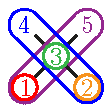
\includegraphics[scale=.8,valign=c]{cyclicOrnamentationX1}\;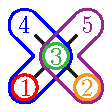
\includegraphics[scale=.8,valign=c]{cyclicOrnamentationX2}
\;\;\text{and}\;\;
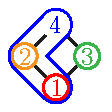
\includegraphics[scale=.8,valign=c]{cyclicOrnamentationD1}\;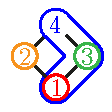
\includegraphics[scale=.8,valign=c]{cyclicOrnamentationD2}\;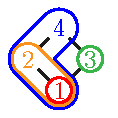
\includegraphics[scale=.8,valign=c]{cyclicOrnamentationD3}\;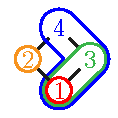
\includegraphics[scale=.8,valign=c]{cyclicOrnamentationD4}
\;\;\text{and}\;\;
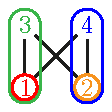
\includegraphics[scale=.8,valign=c]{cyclicOrnamentationT1}\;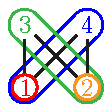
\includegraphics[scale=.8,valign=c]{cyclicOrnamentationT2}\]
since their fibers are all singletons, containing the cyclic reorientations of~$\tc(D)$ given by
\[
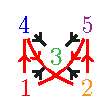
\includegraphics[scale=.8,valign=c]{cyclicReorientationX1}\;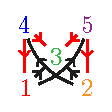
\includegraphics[scale=.8,valign=c]{cyclicReorientationX2}
\;\;\text{and}\;\;
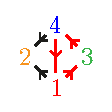
\includegraphics[scale=.8,valign=c]{cyclicReorientationD1}\;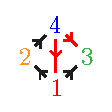
\includegraphics[scale=.8,valign=c]{cyclicReorientationD2}\;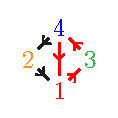
\includegraphics[scale=.8,valign=c]{cyclicReorientationD3}\;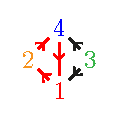
\includegraphics[scale=.8,valign=c]{cyclicReorientationD4}
\;\;\text{and}\;\;
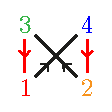
\includegraphics[scale=.8,valign=c]{cyclicReorientationT1}\;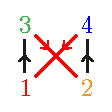
\includegraphics[scale=.8,valign=c]{cyclicReorientationT2}
\]
(in which we have colored a directed cycle in red).
\end{remark}

\begin{proposition}
The map~$S \mapsto \aorn{S}$ is a poset isomorphism from the acyclic sourcing poset~$\ASour(\PP(D))$ to the acyclic ornamentation poset~$\AOrn(D)$.
\end{proposition}

\begin{proof}
By \cref{lem:ASour2AOrn1}, the map~$S \mapsto \aorn{S}$ is injective on acyclic sourcings.

We have seen in \cref{lem:Orn2Sour2} that the map~$O \mapsto \sour{O}$ is a section of the map~$S \mapsto \orn{S}$ on all sourcings.
By definition of acyclic ornamentations, the map~$O \mapsto \asour{O}$ is thus also a section of the map~$S \mapsto \aorn{S}$ on acyclic sourcings.
Hence, the map~$S \mapsto \aorn{S}$ is surjective.

Finally, we have seen that~$S \mapsto \orn{S}$ and~$O \mapsto \sour{O}$ are order-preserving in \cref{lem:Sour2Orn2,lem:Orn2Sour1}.
We conclude that~$S \mapsto \aorn{S}$ and~$O \mapsto \asour{O}$ are inverse isomorphisms from the acyclic sourcing poset~$\ASour(\PP(D))$ to the acyclic ornamentation poset~$\AOrn(D)$.
\end{proof}

%%%%%%%%%%%%%%%%%%%%%%%%%%%%%%%%%%%%%%
%%%%%%%%%%%%%%%%%%%%%%%%%%%%%%%%%%%%%%
%%%%%%%%%%%%%%%%%%%%%%%%%%%%%%%%%%%%%%

\section{Rooted trees}
\label{sec:rootedTrees}

In this section, we discuss the specific situation when the ground graph~$D$ is a rooted tree.

\begin{proposition}
\label{prop:rootedTrees}
Assume that~$T$ is a rooted tree (with increasing edges all oriented toward the root). Then
\begin{enumerate}
\item The acyclic reorientation poset~$\AReori(\tc(T))$, the acyclic sourcing poset~$\ASour(\PP(T))$, and the acyclic ornamentation poset~$\AOrn(T)$ are lattices.
\item All ornamentations of~$T$ are acyclic, so that~$\ASour(\PP(T)) \simeq \AOrn(T) = \Orn(T)$.
\item The map $R \mapsto \asour{R}$ is a surjective lattice map, hence~$\ASour(\PP(T))$ is a lattice quotient~of~$\AReori(\tc(T))$.
\end{enumerate}
\end{proposition}

\begin{proof}
\vincent{todo}
\end{proof}

\begin{corollary}
If~$T$ is a rooted tree, then the Hasse diagram of the ornamentation lattice~$\Orn(T)$ is isomorphic to the graph of the path hypergraphic polytope~$\simplex_{\PP(D)} \eqdef \sum_{u \le_T v} \simplex_{[u,v]_T}$ oriented in the direction~$\omega$.
\end{corollary}

\vincent{This is not completely proved here since I have not proved that the graph is transitively reduced...}

\begin{remark}
Lattice quotients of acyclic reorientation lattices were studied in details in~\cite{Pilaud-acyclicReorientationLattices}.
We can reformulate \cref{prop:rootedTrees} using the language of~\cite{Pilaud-acyclicReorientationLattices}: if~$T$ is a rooted tree with increasing edges all oriented towards the root, then
\begin{enumerate}
\item the transitive closure~$\tc(T)$ is skeletal, so that~$\AReori(\tc(T))$ is an acyclic reorientation lattice,
\item the ornamentation lattice~$\AReori(\tc(T))$ is (isomorphic to) the Tamari lattice of~$\tc(T)$ defined by the $\tc(T)$-sylvester congruence,
\item the path hypergraphic polytope~$\simplex_{\PP(T)}$ is the $\tc(T)$-associahedron.
\end{enumerate}
\end{remark}

\begin{remark}
It might seem more natural to use the map~$\fS_n \to \ASour(\PP(T))$ defined by~$\pi \mapsto \asour{\areori{\pi}}$ instead of the map~$\AReori(\tc(T)) \to \ASour(\PP(T))$ defined by~$R \mapsto \asour{R}$.
However, the former is not always a lattice map, while the latter is.
For instance, the fiber of the ornamentation
...
is the set of permutations~$\{\}$ which is not even an interval of the weak order.
\vincent{todo}
\end{remark}

\begin{example}
Complete binary tree?
\end{example}

\begin{example}
Brooms?
%sage: n = 2 
%....: for m in range(6): 
%....:     print(m, len(digraph_ornamentation_lattice(DiGraph([list(range(n+m)), [(i,n) for i in range(n)] + [(n+j,n+j+Integer(1)) for j in range(m)]])))) 
%....:                                                                                                                                                                                                     
%0 8
%1 13
%2 42
%3 138
%4 462
%5 1573
%A070031
%Expansion of (1+x*C)*C^3, where C = (1-sqrt(1-4*x))/(2*x) is g.f. for Catalan numbers, A000108.

%sage: n = 3 
%....: for m in range(5): 
%....:     print(m, len(digraph_ornamentation_lattice(DiGraph([list(range(n+m)), [(i,n) for i in range(n)] + [(n+j,n+j+Integer(1)) for j in range(m)]])))) 
%....:                                                                                                                                                                                                     
%0 8
%1 35
%2 134
%3 492
%4 1782

%sage: n = 4 
%....: for m in range(4): 
%....:     print(m, len(digraph_ornamentation_lattice(DiGraph([list(range(n+m)), [(i,n) for i in range(n)] + [(n+j,n+j+Integer(1)) for j in range(m)]])))) 
%....:                                                                                                                                                                                                     
%0 16
%1 97
%2 450
%3 1878
\end{example}


%%%%%%%%%%%%%%%%%%%%%%%%%%%%%%%%%%%%%%
%%%%%%%%%%%%%%%%%%%%%%%%%%%%%%%%%%%%%%
%%%%%%%%%%%%%%%%%%%%%%%%%%%%%%%%%%%%%%

\section{Directed trees}
\label{sec:directedTrees}

%%%%%%%%%%%%%%%%%%%%%%%%%%%%%%%%%%%%%%
%%%%%%%%%%%%%%%%%%%%%%%%%%%%%%%%%%%%%%
%%%%%%%%%%%%%%%%%%%%%%%%%%%%%%%%%%%%%%

\section{intreeval hypergraphic lattices}
\label{sec:intreevalHypergraphicPosets}

%%%%%%%%%%%%%%%%%%%%%%%%%%%%%%%%%%%%%%
%%%%%%%%%%%%%%%%%%%%%%%%%%%%%%%%%%%%%%
%%%%%%%%%%%%%%%%%%%%%%%%%%%%%%%%%%%%%%

\section*{Acknowledgments}

This work was initiated at the Banff workshop ``Lattice Theory'' in January 2025.
We are grateful to the organizers (Emily Barnard, Cesar Ceballos, Colin Defant, Osamu Iyama, and Nathan Williams) and to all participants for the friendly and inspiring atmosphere.
We particularly thank Eleni Tzanaki for several conversations on related topics on hypergraphical polytopes.

%%%%%%%%%%%%%%%%%%%%%%%%%%%%%%%%%%%%%%
%%%%%%%%%%%%%%%%%%%%%%%%%%%%%%%%%%%%%%
%%%%%%%%%%%%%%%%%%%%%%%%%%%%%%%%%%%%%%

\bibliographystyle{alpha}
\bibliography{intreevalLattices}
\label{sec:biblio}

%%%%%%%%%%%%%%%%%%%%%%%%%%%%%%%%%%%%%%

\end{document}
